% !TEX root=meca1321-synthesis.tex
\tikzsetnextfilename{PoiseuilleCouetteProfile}
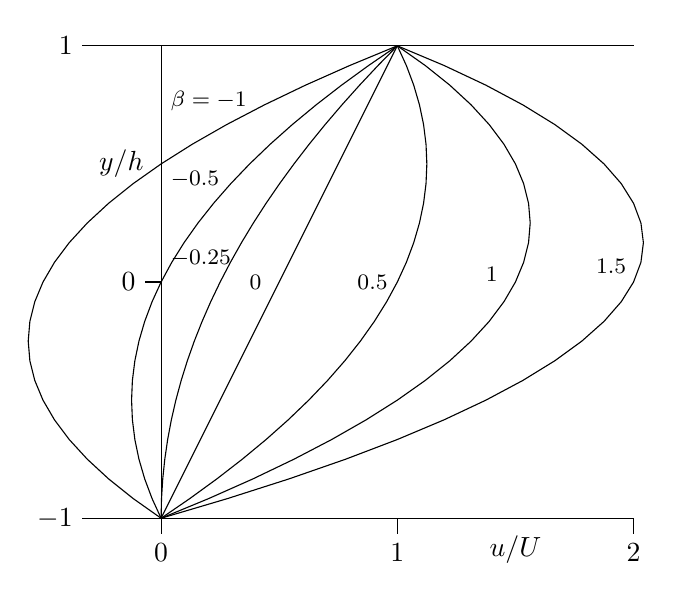
\begin{tikzpicture}
  \draw (-4,-3) -- (3,-3);
  \draw (-4,3) -- (3,3);
  \draw (-3,-3) -- (-3,3);
  \foreach \i in {0,...,2}
  {
    \pgfmathsetmacro{\x}{(-3 + \i*3)};
    \draw (\x,-3) -- ++(0,-0.2);
    \draw (\x,-3.2) node [below] {$\i$};
  }
  \draw (-3,0) -- ++(-0.2,0);
  \draw (-3.2,0) node [left] {$0$};
  \draw (-4,-3) node [left] {$-1$};
  \draw (-4,3) node [left] {$1$};
  \draw (1.5,-3.1) node [below] {$u/U$};
  \draw (-3.1, 1.5) node [left] {$y/h$};

  \foreach \i in {-1,-0.5,-0.25,0,0.5,1,1.5}
  {
    \draw [domain=-1:1] plot ({(\i*(1-(\x)^(2)) + 1/2*(1+\x))*3-3},{\x*3});
  }
  \draw (-3,2.3) node [right] {\footnotesize $\beta=-1$};
  \draw (-3,1.3) node [right] {\footnotesize $-0.5$};
  \draw (-3,0.3) node [right] {\footnotesize $-0.25$};
  \draw (-2,0) node [right] {\footnotesize $0$};
  \draw (0,0) node [left] {\footnotesize $0.5$};
  \draw (1,0.1) node [right] {\footnotesize $1$};
  \draw (2.4,0.2) [right] node {\footnotesize $1.5$};

\end{tikzpicture}
